\chapter{Geografía y teoría económica}

\section{Introdución}

\textbf{La agrupación de actividades económicas se puede encontrar en varios niveles de agregación:} la variación considerable en el tamaño económico de las ciudades o regiones a nivel nacional, o la distribución desigual de la riqueza y la producción a nivel mundial.\\
Surge la pregunta de por qué la ubicación parece ser tan importante para las actividades económicas. Para responder a esta pregunta, necesitamos un marco analítico en el que la geografía juegue un papel de una forma u otra.\\
Las ciudades y regiones varían en tamaño y relevancia. Este es un tema primordial para la economía regional y urbana y también para la geografía económica propiamente dicha, que tradicionalmente se ocupa del análisis teórico de las interdependencias entre ciudades y regiones dentro de un país.\\\\
\begin{center}
    ¿qué tiene que decir cada teoría sobre el papel de la geografía?
\end{center}

\section{La geografía en la economía regional y urbana}
\textbf{La economía regional analiza la dispersión espacial y la coherencia de la actividad económica}
\textbf{La economía regional (también conocida como ciencia regional) se basa en la teoría económica neoclásica y es, en efecto, la sucesora formalizada de la tradición alemana de la economía de ubicación. La geografía económica, por otro lado, es más ecléctica y orientada empíricamente.} Se inspira en teorías económicas heterodoxas y, cada vez más, en áreas externas a la economía, como la sociología, las ciencias políticas y la teoría de la regulación. Comenzamos con una descripción general de un campo de estudio más joven, a saber, \textbf{la economía urbana, que estudia la estructura espacial de las áreas urbanas.} Al igual que la economía regional, la economía urbana se basa en gran medida en las herramientas del análisis neoclásico, de modo que la división entre economía regional y urbana no siempre es clara. 

\subsection{La economía urbana}

\textbf{La distribución desigual de la actividad económica dentro de cada país es el punto de partida de la economía urbana.} El análisis moderno de la aglomeración de empresas y personas en ciudades o áreas metropolitanas se basa en gran medida en \textbf{la economía de la aglomeración, un término que se refiere a la disminución de los costos promedio a medida que se produce una mayor producción dentro de un área geográfica específica. En otras palabras, se basa en rendimientos crecientes a escala.} Antes de entrar en la relevancia de las economías de escala para las ciudades y otras formas de aglomeración, primero analizamos un modelo en el que no hay rendimientos crecientes a escala. Este modelo, el modelo de ciudad monocéntrica. Se justifica una breve discusión, aunque solo sea para poder notar las diferencias con el enfoque de la economía geográfica y dejar claro que, al final, el análisis de las ciudades seguirá siendo bastante limitado mientras no haya rendimientos crecientes a escala.

\subsubsection{El modelo de la ciudad monocéntrica}
El modelo de ciudad monocéntrica asume la existencia de un plano sin rasgos distintivos, perfectamente plano y homogéneo en todos los aspectos. En medio de este plano hay una sola ciudad. Fuera de la ciudad, los agricultores cultivan cultivos que deben vender en la ciudad. Hay costos de transporte positivos asociados con llevar los productos agrícolas a la ciudad, que difieren para los diversos cultivos, al igual que los precios de estos cultivos. Se  analiza cómo los granjeros se ubican a través del plano. \textbf{Cada agricultor quiere estar lo más cerca posible de la ciudad para minimizar sus costos de transporte.} Este incentivo de estar cerca de la ciudad da como resultado mayores rentas de la tierra cerca de la ciudad que en el borde del plano. Por lo tanto, \textbf{cada agricultor se enfrenta a una compensación entre las rentas de la tierra y los costos de transporte.}\\
\textbf{Se demostró que la competencia por las ubicaciones garantiza que la asignación de tierras equilibrada resultante entre los agricultores sea eficiente.} Para cada tipo de cultivo existe una curva de oferta-renta que indica, dependiendo de la distancia a la ciudad, cuánto están dispuestos a pagar los agricultores por la tierra. Dado que las curvas de oferta-renta difieren por cultivo, como resultado de los diferentes precios de esos cultivos en la ciudad y los diferentes costos de transporte, los agricultores de un tipo particular de cultivo pueden superar a sus competidores (es decir, están dispuestos a pagar más) \textbf{para cualquier distancia dada a la ciudad. A medida que nos alejamos del centro de la ciudad,  vemos que, primero, los productores de flores superan la oferta de los otros dos grupos de agricultores, luego que entre los puntos A y B los productores de vegetales están dispuestos a pagar las rentas más altas y que a la derecha del punto B (y por lo tanto el más alejado del centro de la ciudad) los productores de granos pagarán la renta más alta.} Esto da como resultado un patrón de círculos concéntricos de uso de la tierra alrededor de la ciudad, cada anillo consta de granjas que cultivan el mismo cultivo; en secuencia: flores, vegetales y granos.\\
La economía urbana probablemente comenzó como una disciplina separada con William Alonso (1964), quien tomó el modelo de von Thunen y, esencialmente, reemplazó la ciudad por un centro comercial central y los agricultores por viajeros. Los viajeros viajan de ida y vuelta a su trabajo en el centro de negocios, y cada viajero obtiene utilidad de su espacio para vivir, pero también enfrenta costos de transporte. Nuevamente, las rentas de la tierra son las más altas cerca de la ciudad y disminuyen con la distancia. Por lo tanto, se puede aplicar el enfoque de oferta y renta, y la competencia por la tierra entre los viajeros implica una asignación eficiente de la tierra. La eficiencia de la asignación de tierras en el modelo monocéntrico depende del supuesto de que no hay externalidades de ubicación. Combinado con el trabajo de Richard Muth (1969) y Mills (1967), el modelo de Alonso (1964) es sigue siendo la columna vertebral de la economía urbana moderna.\\
Una serie de hechos estilizados sobre la estructura espacial urbana están de acuerdo con el modelo monocéntrico. Primero, la densidad de población disminuye con la distancia de los centros comerciales centrales. En segundo lugar, casi todas las ciudades importantes del mundo occidental se descentralizaron en el siglo XX (a medida que la gente comenzó a ubicarse más lejos del centro de la ciudad), lo que puede estar relacionado con una caída en los costos de transporte. \textbf{El modelo monocéntrico también tiene algunas limitaciones serias. Mencionamos solo dos. Primero, el modelo no tiene en cuenta ninguna interacción entre ciudades; no puede ocuparse de los sistemas urbanos. Segundo, el modelo toma la existencia y ubicación de la ciudad como dadas y se enfoca en la ubicación de agricultores/viajeros fuera de la ciudad.} La pregunta de por qué hay una ciudad para empezar queda sin respuesta. Para hacer frente a estas limitaciones, los economistas urbanos han reconocido durante mucho tiempo que una teoría de las ciudades no puede prescindir de la introducción y el fundamento teórico de algún tipo de rendimientos crecientes a escala. Estos pueden ocurrir a nivel de empresa o a un nivel más agregado (el nivel de la industria o el nivel nacional). 

\paragraph{Economías de escala externas e internas}
\textbf{El término economías de escala o rendimientos crecientes a escala se refiere a una situación en la que un aumento en el nivel de producción implica una disminución en los costos promedio por unidad de producción para la empresa. Se traduce en una curva de costo promedio con pendiente negativa. Para identificar el origen de la caída de los costes medios, se distingue entre economías de escala internas y externas. Con las economías de escala internas, la disminución de los costes medios se produce por un aumento del nivel de producción de la propia empresa.} Cuanto más produce la empresa, mejor puede beneficiarse de las economías de escala y mayor es su ventaja de costos sobre las empresas más pequeñas. \textbf{La estructura de mercado que subyace a las economías de escala internas, típicamente utilizada en la literatura de economía geográfica, debe ser necesariamente de competencia imperfecta, ya que las economías de escala internas implican poder de mercado.} Con \textbf{las economías de escala externas, la disminución de los costes medios se produce a través de un aumento de la producción a nivel de la industria en su conjunto, lo que hace que los costes medios por unidad sean una función de la producción de toda la industria. Scitovsky distingue aquí entre economías externas puras y pecuniarias.}\\
\textbf{Con economías externas puras (o tecnológicas), un aumento en la producción de toda la industria altera la relación tecnológica entre insumos y producción para cada empresa individual. Por lo tanto, tiene un impacto en la función de producción de la empresa.} Un ejemplo de uso frecuente (que se remonta a Alfred Marshall; se refiere a los derrames de información. Un aumento en la producción de la industria aumenta el acervo de conocimiento a través de los efectos indirectos positivos de información para cada empresa, lo que lleva a un aumento en la producción a nivel de empresa. \textbf{En la economía urbana, pero también en la nueva teoría del crecimiento  y la nueva teoría del comercio , se supone que existen economías externas puras. La estructura del mercado puede entonces ser perfectamente competitiva ya que el tamaño de la empresa individual no importa.}\\
\textbf{Las economías externas pecuniarias son transmitidas por el mercado a través de efectos de precio para la empresa individual, lo que puede alterar su decisión de producción.} Dos ejemplos, de nuevo basados en Marshall, son la existencia de un gran mercado local de insumos especializados y la puesta en común del mercado laboral. Una gran industria puede respaldar un mercado de insumos intermedios especializados y un grupo de trabajadores calificados específicos de la industria, lo que beneficia a la empresa individual. \textbf{A diferencia de las economías externas puras, estos efectos indirectos no afectan la relación tecnológica entre insumos y productos (la función de producción). Las externalidades pecuniarias existen en la literatura de economía geográfica a través de un efecto de gusto por la variedad en un gran mercado local. La utilidad de cada consumidor depende positivamente del número de variedades que puede comprar de un bien manufacturado. Los efectos de precio cruciales para las externalidades pecuniarias solo pueden ocurrir con competencia imperfecta. Esto es consistente con el requisito de competencia imperfecta para las economías de escala internas, también utilizado en la literatura de economía geográfica.}\\
Algunas observaciones finales están en orden. Primero, los derrames o externalidades son cruciales para las economías externas. El concepto de derrames a veces se utiliza solo para economías externas puras, refiriéndose a las economías externas pecuniarias como un caso de interdependencia del mercado. Nos ceñimos al uso de derrames o externalidades cuando nos referimos a economías de escala externas en general. De manera similar, el término rendimientos crecientes a veces se usa solo para economías de escala internas. También usamos la frase rendimientos crecientes cuando hablamos de economías externas. Del contexto quedará claro si nos referimos al nivel de la empresa o de la industria.\\

\begin{center}
    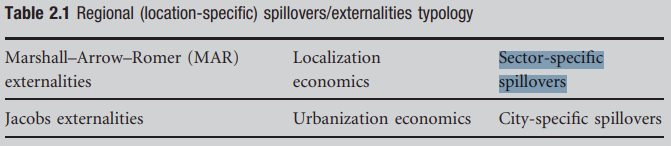
\includegraphics[scale=0.5]{imagen/imagen1.png}
\end{center}

\textbf{En segundo lugar, las economías externas pueden aplicarse a un nivel de agregación superior al de la empresa. Este suele ser el nivel de la industria, pero en la teoría moderna del comercio y la teoría moderna del crecimiento también puede ser la economía en su conjunto. Tercero, las economías externas en los modelos son estáticas, mientras que la literatura también considera economías externas dinámicas.} En ese caso, los costos promedio por unidad de producción son una función negativa de la producción acumulada de la industria. Nuevamente, si esto es relevante, quedará claro si nos referimos a economías externas estáticas o dinámicas. \textbf{Cuarto, las economías externas discutidas anteriormente son positivas,  también pueden ser negativos, es decir, un aumento en la producción de una empresa conduce a un aumento en los costos por unidad para otras empresas.}\\
Finalmente, una observación sobre la terminología un tanto confusa con respecto a las externalidades económicas regionales o efectos indirectos. Es habitual distinguir entre las externalidades Marshall-Arrow-Romer (MAR) y las externalidades de Jacobs. En ambos casos, el énfasis está en los efectos indirectos regionales (específicos de la ubicación), es decir, las empresas deben estar ubicadas lo suficientemente cerca unas de otras para beneficiarse de estas externalidades. Las externalidades SAM se centran en los efectos indirectos específicos del sector y también se conocen como economía de localización. Las externalidades de Jacobs se centran en los efectos indirectos específicos de la ciudad que cruzan los límites entre sectores individuales. Estos también se conocen como economía de la urbanización. 


\subsubsection{Economía urbana y rendimientos crecientes}
\textbf{A diferencia del modelo de ciudad monocéntrica, se incluyen rendimientos crecientes a escala. El punto de partida es bastante diferente del modelo monocéntrico. No hay costes de transporte y el interior de una ciudad ya no forma parte del análisis.} En cierto sentido, es un análisis de las ciudades en las que el espacio, es decir, el espacio fuera de las ciudades, no tiene ningún papel que desempeñar. \textbf{La justificación de este descuido geográfico del espacio no urbano es que, en los países industrializados modernos, una gran parte de la actividad económica general y de la población se encuentra en áreas urbanas, de modo que la relevancia de lo urbano frente a lo no urbano Se supone que las transacciones son limitadas.} En cambio, \textbf{el análisis se centra en las fuerzas que determinan el tamaño de las ciudades y las interacciones entre ellas. Las fuerzas de aglomeración en el modelo de Henderson son economías de escala externas positivas que son específicas de la industria. Esto último significa que hay derrames positivos cuando una empresa de una industria en particular se ubica en una ciudad donde se encuentran otras empresas de la misma industria.} Usando una categorización bien conocida que se remonta a los trabajos de Marshall, estos pueden deberse a:
\begin{enumerate}[\bfseries (i)]
    \item El intercambio de información, 
    \item la existencia de una gran cantidad de mano de obra, o
    \item la existencia de especialistas proveedores.
\end{enumerate}
Por lo tanto, las economías externas pueden, en principio, involucrar economías externas puras (como en el enfoque original de Henderson) o economías externas pecuniarias. \\
Las fuerzas de expansión son economías de escala externas negativas dentro de la ciudad, como la congestión, que es una función del tamaño total de la ciudad. Una ciudad grande implica costos de transporte y rentas de la tierra relativamente altos. Las deseconomías de escala no dependen del tipo de producción que se lleva a cabo en la ciudad, por lo que dependen únicamente del tamaño total de una ciudad. Junto con las economías externas específicas de la industria, esto tiene dos implicaciones importantes. En primer lugar, puede racionalizar los sistemas de ciudades (diferentes tamaños de ciudades que satisfacen las necesidades de diferentes industrias). Basado en el supuesto de que los efectos secundarios positivos de la ubicación son específicos de la industria, cada industria tiene su propio tamaño óptimo. Ciudades de diferentes tamaños comercian entre sí. En comparación con el marco de von Thunen o Alonso, la economía urbana moderna es mucho menos ad-hoc porque puede brindar una base teórica para los rendimientos crecientes que impulsan la existencia de las ciudades, y produce conocimientos sobre los sistemas urbanos. 

\subsubsection{¿Qué tipo de economías de escala externas?}
Existe un amplio respaldo empírico para la idea de que los efectos indirectos específicos de la industria son importantes para las ciudades. \textbf{Estas economías externas específicas de la industria se conocen como economías de localización, a diferencia de las economías de urbanización. Las últimas son economías externas que se aplican a empresas de todos los sectores y captan la noción de efectos indirectos positivos para una empresa como resultado de la actividad económica total en una ciudad. Ambos tipos de economías externas a menudo se relacionan con la ubicación de las ciudades en un sentido estático, pero también se aplican en un contexto dinámico (¿cómo se desarrollan las ciudades con el tiempo?).} Con respecto al crecimiento de las ciudades en los Estados Unidos, no encuentran apoyo para la hipótesis de que las ciudades especializadas en ciertas industrias crecen más rápidamente en promedio. En cambio, concluyen que \textbf{si las economías externas son importantes, probablemente sea más importante tener una variedad de industrias diversificadas en una ciudad.} Si este último es el caso, surge la pregunta de por qué tantas ciudades están especializadas en industrias particulares. Se sugieren que tanto las economías de localización como las de urbanización son relevantes (aunque al final favorecen las economías de urbanización), mientras que otros argumentan que en un contexto dinámico las economías de localización son más relevantes.\\
Desde un punto de vista teórico, cabe destacar que el enfoque de los sistemas urbanos de Henderson no da por sentada la existencia de la ciudad, como hacía el modelo monocéntrico. También proporciona una teoría de las interacciones entre ciudades. \textbf{El problema con el enfoque es que el espacio fuera de las ciudades (deliberadamente) no forma parte del análisis. Esto es problemático si uno quiere poder decir dónde están ubicadas las ciudades en relación con otras y la parte no urbana de la geografía:} La literatura sobre sistemas de ciudades ha enfatizado el espacio urbano pero ha descuidado el espacio nacional. Como veremos, \textbf{la ubicación de la actividad manufacturera y la relación entre estas ubicaciones y el resto del espacio es un tema clave en la economía geográfica. Para analizar esta relación, los costos de transporte deben ser parte del análisis, ya que son cruciales para determinar el equilibrio entre las fuerzas de aglomeración y expansión.}\\
En sus estudios de las teorías de la aglomeración, que incluye la economía urbana, \textbf{se analizan tres enfoques básicos: rendimientos crecientes, externalidades y competencia espacial.} Su uso de rendimientos crecientes y externalidades corresponde a nuestra definición de economías externas puras y economías externas pecuniarias, respectivamente. Ambos tipos de economías externas son importantes. Esto deja la competencia espacial, lo que significa que \textbf{la competencia entre empresas es casi automáticamente de naturaleza oligopólica cuando se toma en consideración el espacio.} La competencia está restringida por la distancia; Por lo general, se piensa que una empresa compite solo con sus empresas vecinas. \textbf{La competencia espacial está, por tanto, intrínsecamente ligada al comportamiento estratégico de las empresas. La razón es simplemente que en la economía geográfica y en particular en la versión de competencia monopolística, que caracteriza la estructura del mercado en nuestro modelo central de economía geográfica, el comportamiento estratégico no es tenido en cuenta.} Las empresas toman el comportamiento (fijación de precios) de las demás como dado. Además de los tres enfoques mencionados dan dos razones adicionales para la aglomeración (urbana): la existencia de un espacio no homogéneo y economías de escala internas en un proceso de producción. Con el primero se puede racionalizar la aglomeración sin ninguna forma de rendimientos crecientes a escala (piense en las diferencias en la geografía física real que da lugar, por ejemplo, a un puerto natural y la aglomeración correspondiente).

\subsection{Economía regional}
\textbf{La economía regional analiza la organización espacial de los sistemas económicos (y no solo de las ciudades) y de alguna manera también debe dar cuenta de la distribución desigual en el espacio.} Todas las contribuciones alemanas toman en consideración el espacio nacional o de toda la economía para analizar dónde se ubican las actividades económicas. Esta es una pregunta relevante ya que el movimiento de bienes y personas no es gratuito y la producción suele estar sujeta a alguna forma de rendimientos crecientes. Sin embargo, los padres fundadores de la economía regional se centran en diferentes aspectos de la ubicación de la actividad económica. Como vimos, von Thunen, por ejemplo, enfatizó las decisiones de ubicación tomadas por los agricultores, mientras que Weber analizó la ubicación óptima y el tamaño de la planta para las empresas manufactureras. Esta subsección se centra en las ideas presentadas (y probadas) por primera vez por Christaller y Losch, quienes trataron no solo de explicar la ubicación de las ciudades sino también de diferenciarlas por las diversas funciones que desempeñan y de tratar las relaciones entre las ciudades y el medio ambiente. No ciudades. Este enfoque se conoce como la teoría del lugar central, que muestra que diferentes puntos o ubicaciones en el panorama económico tienen diferentes niveles de centralidad y que los bienes y servicios se proporcionan de manera eficiente sobre una base jerárquica.\\

\subsubsection{Teoría del lugar central}
\textbf{Dada una distribución uniforme de consumidores idénticos en un plano homogéneo, la teoría del lugar central sostiene que las ubicaciones difieren en centralidad y que esta centralidad determina el tipo de bienes que proporciona la ubicación.} La provisión de estos bienes está determinada por rendimientos internos crecientes a escala, mientras que la ubicación es relevante porque los consumidores incurren en costos de transporte. Para minimizar estos costos, los consumidores quieren tener acceso a proveedores de bienes cercanos. Para algunos tipos de bienes, como el pan, esto es más fácil que para otros, como los televisores, porque los rendimientos crecientes a escala son relativamente limitados. Por lo tanto, la economía puede sustentar muchos lugares relativamente pequeños (pueblos) donde los panaderos están activos para suministrar pan. Por el contrario, solo puede haber relativamente pocos lugares (ciudades pequeñas, los lugares centrales) donde las empresas de electrónica vendan televisores, que la gente compra con menos frecuencia. Para minimizar los costos de transporte, ambos tipos de ubicaciones se distribuyen de manera bastante uniforme en el espacio. Además, obtenemos una jerarquía de lugares donde la ciudad realiza todas las funciones (vende pan y televisores), mientras que el pueblo realiza solo algunas funciones (vende solo pan). Donde el lugar central equidistante está rodeado por seis equidistantes ciudades más pequeñas, que juntas forman un hexágono. Cada ciudad pequeña, a su vez, está rodeada por seis aldeas equidistantes.\\
El hecho de que se ocupe explícitamente de la ubicación de la actividad económica es una ventaja importante de la teoría del lugar central. El principal problema con el enfoque es que la lógica económica detrás de las decisiones de los consumidores y las empresas sigue sin estar clara. ¿Qué tipo de comportamiento de los agentes individuales conduce a un resultado de lugar central? Los rendimientos crecientes a nivel de empresa requieren alguna forma de competencia imperfecta, un análisis que falta. En consecuencia, la teoría del lugar central, especialmente la versión gráfica que todavía se encuentra en la mayoría de los libros de texto de introducción a la geografía económica, es más una historia descriptiva que un modelo causal.\\
Por supuesto, los científicos regionales y los geógrafos económicos también han sido conscientes de las limitaciones de esta versión de la teoría del lugar central, que durante los últimos treinta años ha recibido menos interés, particularmente dentro de la geografía económica. Para una base teórica, los geógrafos económicos han comenzado a buscar en otra parte. Y también explicamos por qué los geógrafos económicos modernos son bastante críticos con el trabajo realizado por los economistas geográficos (y viceversa). Sin embargo, siguiendo a Walter Isard (1956, 1960), los científicos regionales han tratado de construir sobre las ideas básicas de la teoría del lugar central para dar una base económica teórica (a menudo altamente formalizada) a esta teoría. Estos modelos son en su mayoría de naturaleza de equilibrio parcial, explicando algunos aspectos del sistema de lugar central mientras ignoran otros. \textbf{Por lo general, un modelo en esta tradición no trata con empresas o consumidores individuales, sino que formaliza esencialmente el patrón geométrico de un sistema de lugar central}. El resultado del lugar central es, por lo tanto, meramente racionalizado y no explicado por el comportamiento subyacente de los consumidores y productores, ni por sus decisiones e interacciones (de mercado). Por ejemplo, la curva de demanda que enfrenta una empresa en un lugar particular no se deriva de los primeros principios, sino que simplemente se supone. \textbf{La economía geográfica intenta llenar este vacío en la literatura dando una base microeconómica a la jerarquía de los lugares centrales.} 

\paragraph{Teoría del lugar central en un pólder holandés}

